\PassOptionsToPackage{subsection=false}{beamerouterthememiniframes}
\documentclass{beamer}
%\useoutertheme[footline=authorinstitutetitle, subsection=false]{miniframes}
\usetheme{Berlin}
%\useoutertheme[subsection=false]{miniframes}
\setbeamertemplate{navigation symbols}{}

\title{Reading Digits with Neural Networks}
\author[Todd Sierens]{Todd Sierens\inst{1,2}}
\institute[Perimeter Institute for Theoretical Physics]{\inst{1}Perimeter Institute for Theoretical Physics \\ \inst{2}University of Waterloo}
\date{February 16, 2016}

\usepackage{amsmath}
\usepackage{amssymb}
\usepackage{epstopdf}
\usepackage{xfrac}
%\usepackage{biblatex}
\usepackage[backend=bibtex]{biblatex} 
%\usepackage{subfigure}
\usepackage{subcaption} 
\newcommand{\bs}{\boldsymbol}
\newcommand{\pl}{\ell_P}
%\makeatletter
%    \newenvironment{withoutheadline}{
%        \setbeamertemplate{headline}[default]
%        \def\beamer@entrycode{\vspace*{-\headheight}}
%    }{}
%\makeatother


%\newcounter{savedenum}
%\newcommand*{\saveenum}{\setcounter{savedenum}{\value{enumi}}}
%\newcommand*{\resumeenum}{\setcounter{enumi}{\value{savedenum}}}


%\usepackage{setspace}
%\usepackage{bbm}
%\usepackage{relsize}
%\usepackage{graphicx}
%\usepackage[font=small,labelfont=bf,margin=1.5cm]{caption}
%\usepackage{subcaption}
%\usepackage{listings}

%\hyphenpenalty = 7000
%\tolerance = 1000
\begin{document}

\begin{frame}[plain] 
\titlepage
\end{frame}

\begin{frame}[plain]{Outline}
\tableofcontents
\end{frame}


\section{Handwritten digits}


\begin{frame}[plain]{Handwritten digits}
\begin{figure}
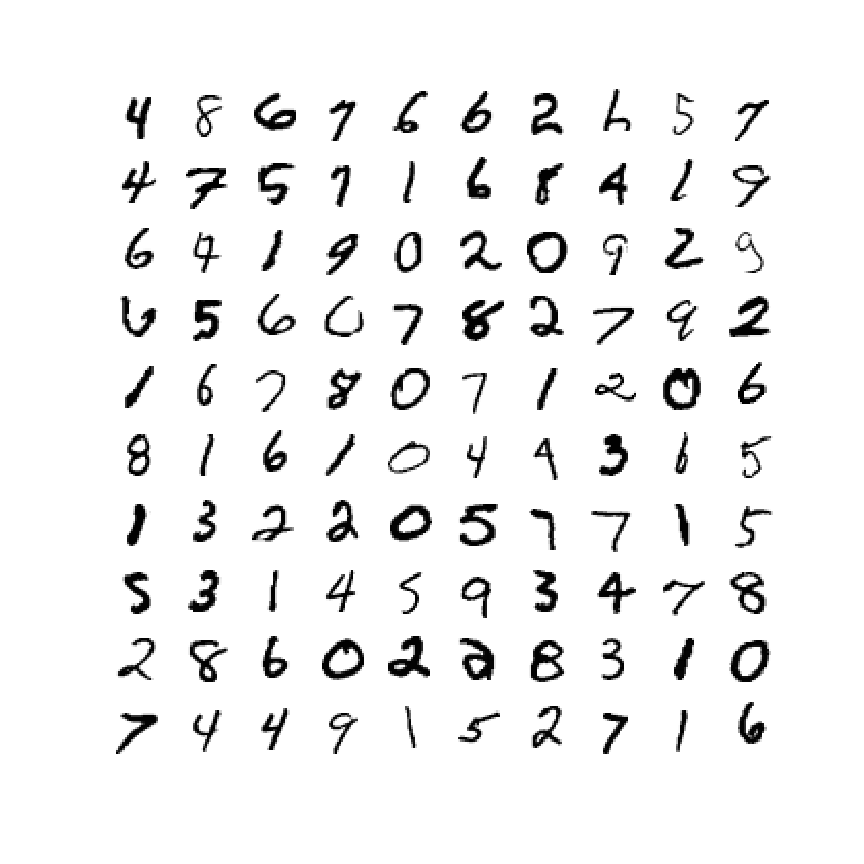
\includegraphics[width=0.7\textwidth]{handwritten_digits}
\vspace{-1cm}
\caption{\centering100 handwritten digits from the MNIST database provided as a training set by kaggle.com.}
\end{figure}
\end{frame}


\section{Neural Network}


\begin{frame}[plain]{Neural Network}
\begin{figure}
\includegraphics[width = 0.8 \textwidth]{"simple neural net no lines"}
\end{figure}
\end{frame}


\begin{frame}[plain]{Neural Network}
\begin{figure}
\includegraphics[width = 0.8 \textwidth]{"simple neural net half lines"}
\end{figure}
\end{frame}


\begin{frame}[plain]{Neural Network}
\begin{figure}
\includegraphics[width = 0.8 \textwidth]{"simple neural net all lines"}
\end{figure}
\end{frame}


\begin{frame}[plain]
\begin{figure}\vspace{-0.5cm}
\begin{subfigure}{0.90\textwidth}
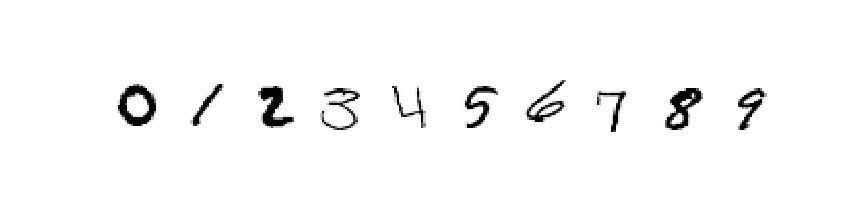
\includegraphics[width=\textwidth]{nn_demo_input_grey}
\caption{Greyscale images of some of the training data.}
\end{subfigure}\\
\begin{subfigure}{0.90\textwidth}
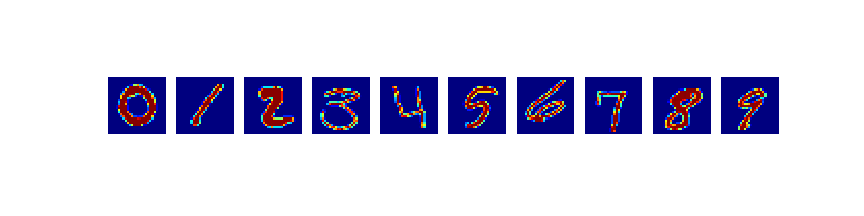
\includegraphics[width=\textwidth]{nn_demo_input}
\caption{Raw input layer of neural network.}
\end{subfigure}\\
\begin{subfigure}{0.90\textwidth}
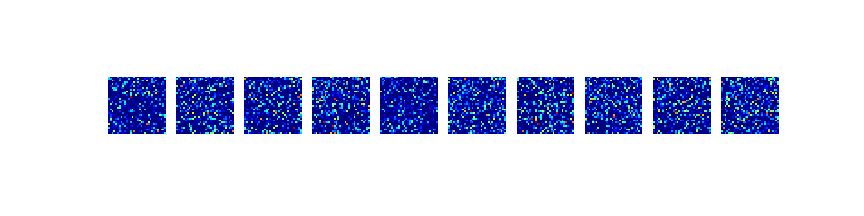
\includegraphics[width=\textwidth]{nn_demo_hidden}
\caption{Hidden layer of neural network.}
\end{subfigure}
\end{figure}
\end{frame}


\section{Multilayer Perceptron}


\begin{frame}[plain]{Multilayer Perceptron}
\begin{figure}
\includegraphics[width = 0.8 \textwidth]{"mlp all lines"}
\end{figure}
\end{frame}

\begin{frame}[plain]
\begin{figure}\vspace{-1.5cm}
\begin{subfigure}{0.2\textwidth}

\includegraphics[width=\textwidth]{mlp_input}

\end{subfigure}
\begin{subfigure}{0.2\textwidth}
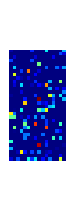
\includegraphics[width=\textwidth]{mlp_1_hidden}

\end{subfigure}
\begin{subfigure}{0.2\textwidth}
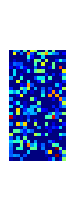
\includegraphics[width=\textwidth]{mlp_2_hidden}
\end{subfigure}
\\\vspace{-1cm}
\begin{subfigure}{0.8\textwidth}
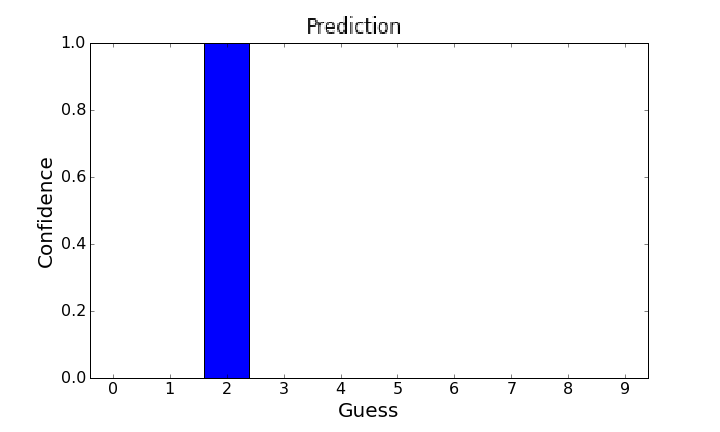
\includegraphics[width=\textwidth]{mlp_prediction}

\end{subfigure}
\end{figure}
\end{frame}


\section{Convolutional Neural Network}


\begin{frame}[plain]{Convolutional Neural Network}
\begin{figure}
\includegraphics[width = 0.8 \textwidth]{"cnn"}
\end{figure}
\end{frame}

\begin{frame}[plain]
\begin{figure}
\begin{subfigure}{0.1\textwidth}

\includegraphics[width=\textwidth]{cnn_input}
\end{subfigure}
\begin{subfigure}{0.3\textwidth}
\caption*{Input Layer}
\end{subfigure}
\\
\begin{subfigure}{0.6\textwidth}
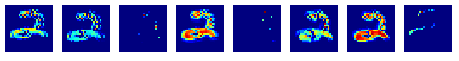
\includegraphics[width=\textwidth]{cnn_1_conv}
\end{subfigure}
\begin{subfigure}{0.3\textwidth}
\caption*{1st conv. layer}
\end{subfigure}
\\
\begin{subfigure}{0.6\textwidth}
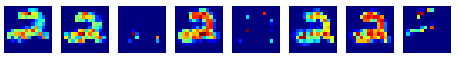
\includegraphics[width=\textwidth]{cnn_1_pool}
\end{subfigure}
\begin{subfigure}{0.3\textwidth}
\caption*{1st pooling layer}
\end{subfigure}
\\
\begin{subfigure}{0.6\textwidth}
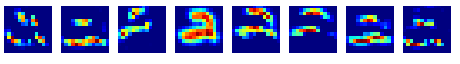
\includegraphics[width=\textwidth]{cnn_3_conv}
\end{subfigure}
\begin{subfigure}{0.3\textwidth}
\caption*{2nd conv. layer}
\end{subfigure}
\\
\begin{subfigure}{0.6\textwidth}
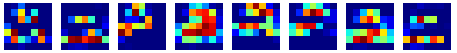
\includegraphics[width=\textwidth]{cnn_2_pool}
\end{subfigure}
\begin{subfigure}{0.3\textwidth}
\caption*{2nd pooling layer}
\end{subfigure}
\\
\begin{subfigure}{0.1\textwidth}
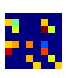
\includegraphics[width=\textwidth]{cnn_hidden}
\end{subfigure}
\begin{subfigure}{0.3\textwidth}
\caption*{Hidden layer}
\end{subfigure}
\\\vspace{-0.2cm}
\begin{subfigure}{0.55\textwidth}
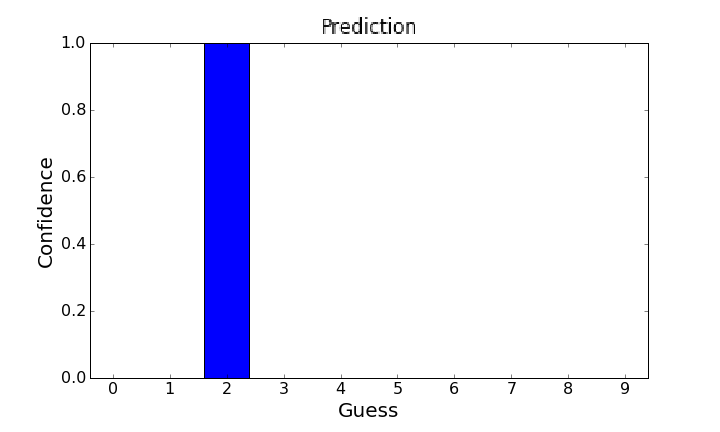
\includegraphics[width=\textwidth]{cnn_prediction}
\end{subfigure}
\begin{subfigure}{0.3\textwidth}
\caption{prediction}
\end{subfigure}


\end{figure}
\end{frame}


\begin{frame}[c]
\begin{itemize}
\centering
\item A deeper convolutional neural network (CNN)
\end{itemize}
\end{frame}


\begin{frame}[plain]
\begin{figure}
\begin{subfigure}{0.1\textwidth}
\caption*{Input}
\end{subfigure}
\begin{subfigure}{0.1\textwidth}

\includegraphics[width=\textwidth]{deep_cnn_input}
\end{subfigure}
\\
\begin{subfigure}{0.1\textwidth}
\caption*{Conv1}
\end{subfigure}
\begin{subfigure}{0.3\textwidth}
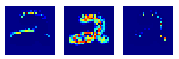
\includegraphics[width=\textwidth]{deep_cnn_1_conv}
\end{subfigure}
\hspace{1cm}
\begin{subfigure}{0.3\textwidth}
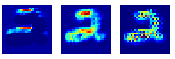
\includegraphics[width=\textwidth]{deep_cnn_2_conv}
\end{subfigure}
\begin{subfigure}{0.1\textwidth}
\caption*{Conv2}
\end{subfigure}
\\
\begin{subfigure}{0.1\textwidth}
\caption*{pool1}
\end{subfigure}
\begin{subfigure}{0.3\textwidth}
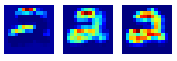
\includegraphics[width=\textwidth]{deep_cnn_1_pool}
\end{subfigure}
\hspace{1cm}
\begin{subfigure}{0.3\textwidth}
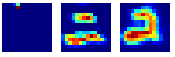
\includegraphics[width=\textwidth]{deep_cnn_3_conv}
\end{subfigure}
\begin{subfigure}{0.1\textwidth}
\caption*{Conv3}
\end{subfigure}
\\
\begin{subfigure}{0.1\textwidth}
\caption*{Conv4}
\end{subfigure}
\begin{subfigure}{0.3\textwidth}
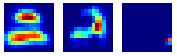
\includegraphics[width=\textwidth]{deep_cnn_4_conv}
\end{subfigure}
\hspace{1cm}
\begin{subfigure}{0.3\textwidth}
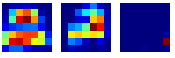
\includegraphics[width=\textwidth]{deep_cnn_2_pool}
\end{subfigure}
\begin{subfigure}{0.1\textwidth}
\caption*{pool2}
\end{subfigure}
\\
\begin{subfigure}{0.1\textwidth}
\caption*{hidden}
\end{subfigure}
\begin{subfigure}{0.1\textwidth}
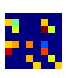
\includegraphics[width=\textwidth]{cnn_hidden}
\end{subfigure}
\\\vspace{-0.2cm}
\begin{subfigure}{0.55\textwidth}
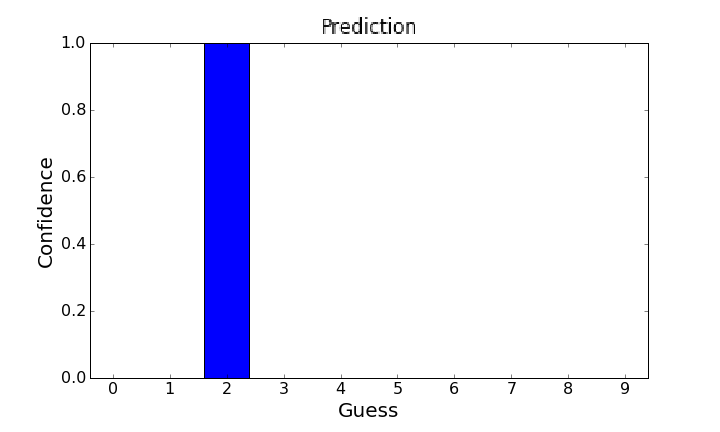
\includegraphics[width=\textwidth]{cnn_prediction}
\end{subfigure}
\end{figure}
\end{frame}


\begin{frame}[plain]
\begin{figure}

\includegraphics[width = 0.5\textwidth]{wrong_guess_pic}
\end{figure}

\begin{figure}
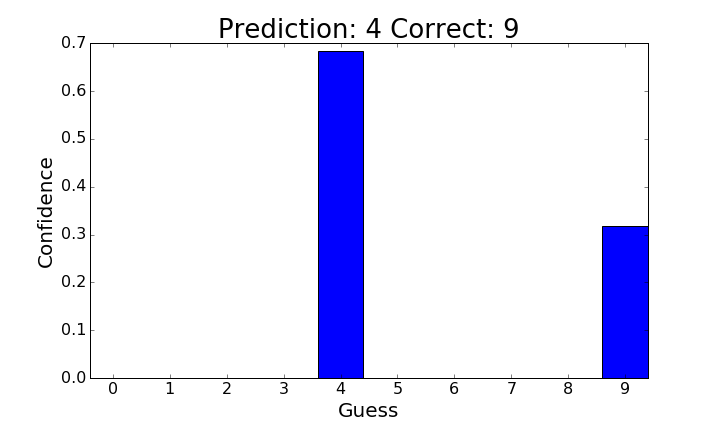
\includegraphics[width = 0.8\textwidth]{wrong_guess2}
\end{figure}
\end{frame}

\section{Performance Metrics}
\begin{frame}[plain]{Performance Metrics}
\begin{figure}
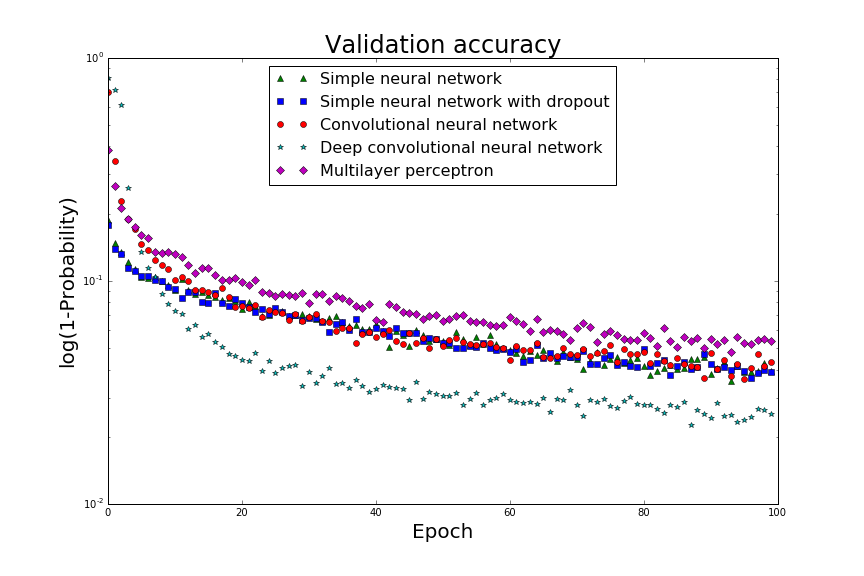
\includegraphics[width = 0.7\textwidth]{log_val_acc}
\caption{The validation accuracy of several models as a function of 'epoch'. }
\end{figure}
\end{frame}

\begin{frame}[plain]{Performance Metrics}
\begin{figure}
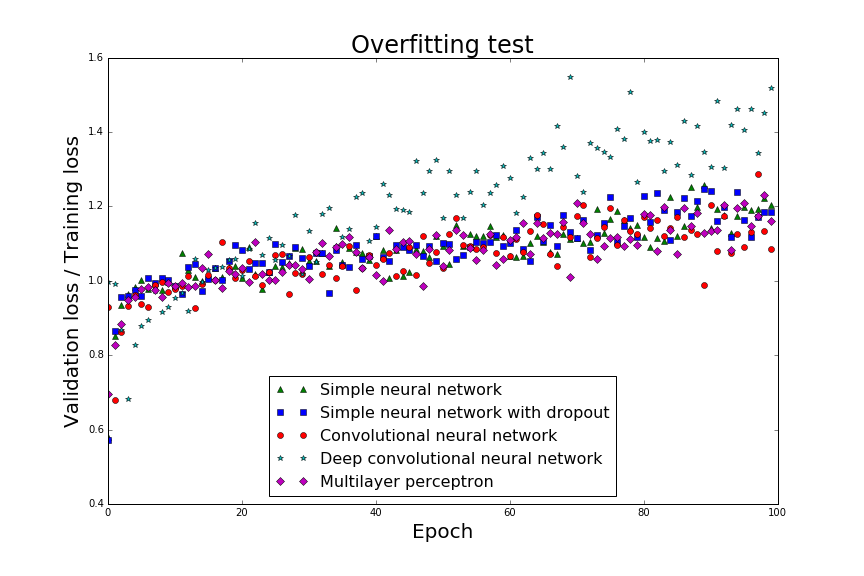
\includegraphics[width = 0.7\textwidth]{ratio}
\caption{A measure of over-fitting. If this value is too far from 1 the model is over-fitting.}
\end{figure}
\end{frame}

\begin{frame}[plain]{Performance Metrics}
\begin{figure}
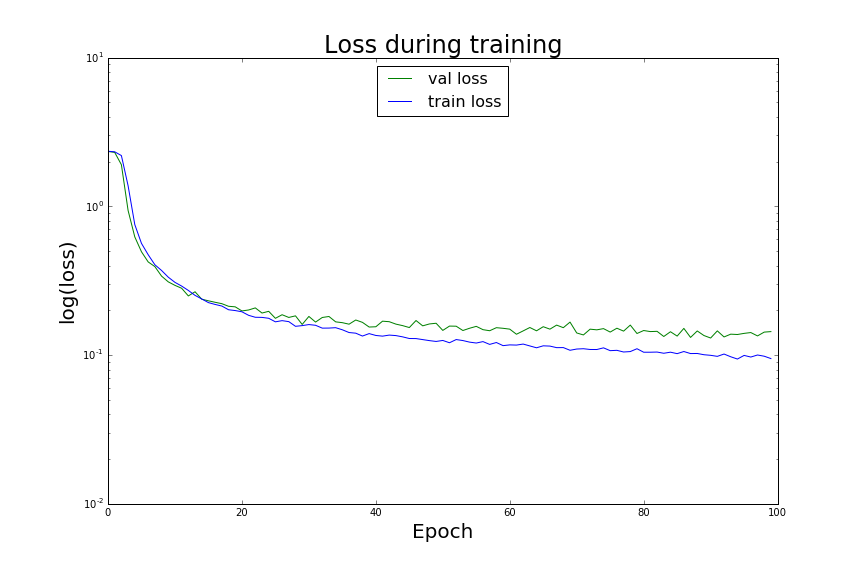
\includegraphics[width = 0.7\textwidth]{cnn_loss}
\caption{Validation loss and training loss for the deep CNN model.}
\end{figure}
\end{frame}

\begin{frame}[plain]{Performance Metrics}
\begin{figure}
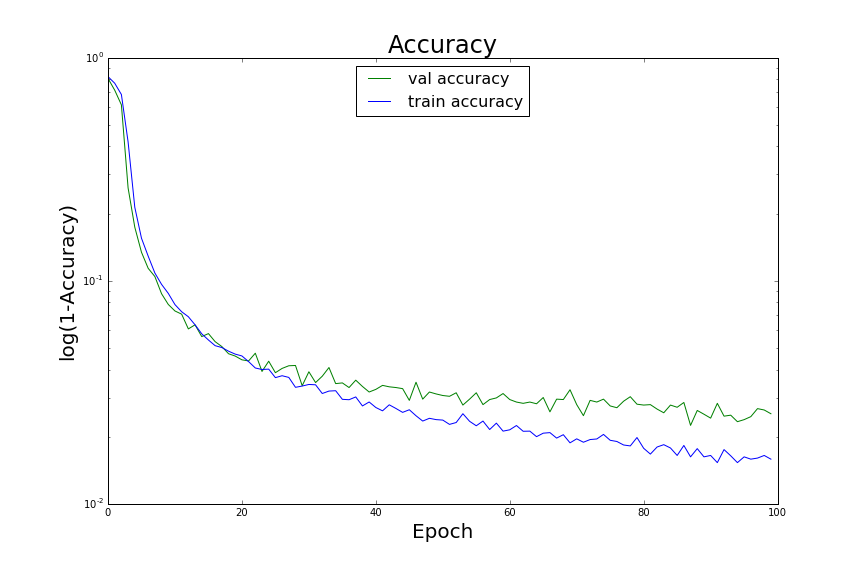
\includegraphics[width = 0.7\textwidth]{cnn_accuracy}
\caption{Validation accuracy and Training accuracy for the deep CNN model.}
\end{figure}
\end{frame}

\begin{frame}[plain]{Performance Metrics}
\begin{figure}
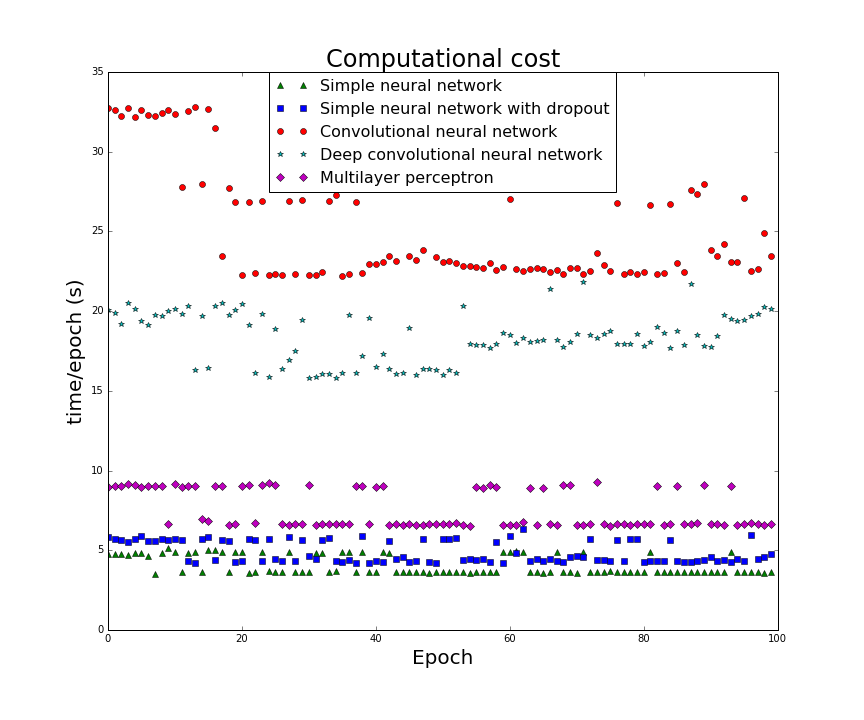
\includegraphics[width = 0.7\textwidth]{comp}
\caption{The amount of time each epoch required to execute. Since performance is dependent on many factors, only the relative time is meaningful.}
\end{figure}
\end{frame}

\section{The End}
\begin{frame}[c]{The End}\centering
\huge The End
\end{frame}

\end{document}